\skriptsection{AM (Amplitudenmodulation)}{43}
Bei der Amplitudenmodulation ist die Amplitude des Trägersignals $A(t)$ linear von der dem
Nachrichtensignal $m(t)$ abhängig.

$$ x_c(t) = A(t) \cos(w_c t) $$




\skriptsubsection{DSB(-SC): Doppelseitenband (Double-Sideband)-AM}{44}
Bei der Doppelseitenband-Amplitudenmodulation ist das untere Seitenband (Lower
Sideband) sowie das
obere Seitenband (Upper Sideband) präsent. Da der Träger im Spektrum nicht
präsent ist, ist bei dieser Art von AM auch von \textbf{DSB-SC (Double-Sideband Suppressed Carrier)} die Rede. \\ 
Die \textbf{Bandbreite} berechnet sich dadurch wie folgt: $ \qquad W_B = 2 w_{\omega}$

\subsubsection{Modulation}
\begin{minipage}[c][2.7cm][t]{6.5cm}
    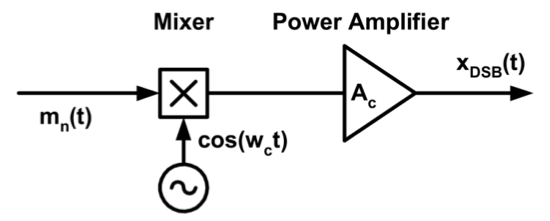
\includegraphics[width=6cm]{bilder/am_dsb_modulation.png}
\end{minipage}
\begin{minipage}[c][2.7cm][t]{11.5cm}
Bei der Doppelseitenband AM wird das Nachrichtensignal mit dem sinusförmigen Trägersignal
multipliziert, wodruch sich dank dem Modulationssatz folgendes Spektrum ergibt. \\
$$ x_{DSB}(t) =
m(t) \cos(w_c t) \quad \laplace \quad X_{DSB} = \frac{1}{2}M(\omega - \omega_c) + \frac{1}{2}M(\omega + \omega_c)$$
\end{minipage}

\begin{minipage}[t]{9.5cm}
    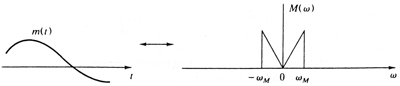
\includegraphics[width=9cm]{bilder/am_dsb_nachrichtensignal.png}
\end{minipage}
\begin{minipage}[t]{9cm}
    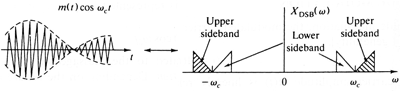
\includegraphics[width=9cm]{bilder/am_dsb_spektrum.png}
\end{minipage}

\subsubsection{Demodulation} 
\label{am_dsb_modulation}
\begin{minipage}[t][2.3cm][c]{6.5cm}
    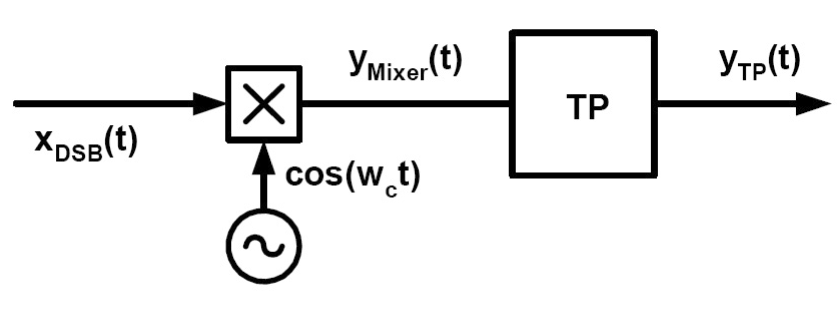
\includegraphics[width=6cm]{bilder/am_dsb_demodulation.png}
\end{minipage}
\begin{minipage}[t][2.3cm][c]{11.5cm}
	Das DSB-Signal wird mit einem sogenannten \textbf{synchronen Demodulator} oder \textbf{koharänten
	Demodulator} zurückgewonnen. Hierbei wird das DSB-Signal mit dem lokalen Träger
	multipliziert und anschliessend das Nachrichtensignal mittels einem Tiefpassfilter rausgefiltert.
	\\ Weicht die Frequenz oder die Phase des lokalen Trägers von deren, des ursprünglichen Trägers ab, 
	so ergeben sich Abschwächungen im demodulierten Nachrichtensignal.
\end{minipage}

\paragraph{Auswirkungen einer Phasenabweichung um $\phi$:} $y_{TP}(t) = \frac{1}{2}
m(t) \cos(-\phi)= \frac{1}{2} m(t) \cos(\phi) $
\paragraph{Auswirkungen einer Frequenzabweichung um $\Delta \omega$:} $y_{TP}(t) =
\frac{1}{2} m(t) \cos(\Delta \omega t)$\\



\skriptsubsection{AM: Gewöhnliche(Ordinary)-AM}{45}
Die gewöhnliche AM wird generiert, indem man dem DSB-Signal ein grosses Trägersignal dazuaddiert.

\subsubsection{Modulation}

$x_{AM}(t) = A_C (1 + \mu \cdot m(t)) \cos(\omega_c t)
	\quad \laplace \quad X_{AM}(\omega) = \frac{1}{2}M(\omega - \omega_c) + \frac{1}{2}M(\omega + \omega_c) + \pi A_C [\delta (\omega - \omega_c) + \delta (\omega + \omega_c)]$
	$m(t) \laplace M(\omega)$ \\
	$\mu \cdot sin(\omega t) \laplace \pi \cdot \mu \cdot \delta(\omega)$

\begin{minipage}[]{9cm}
	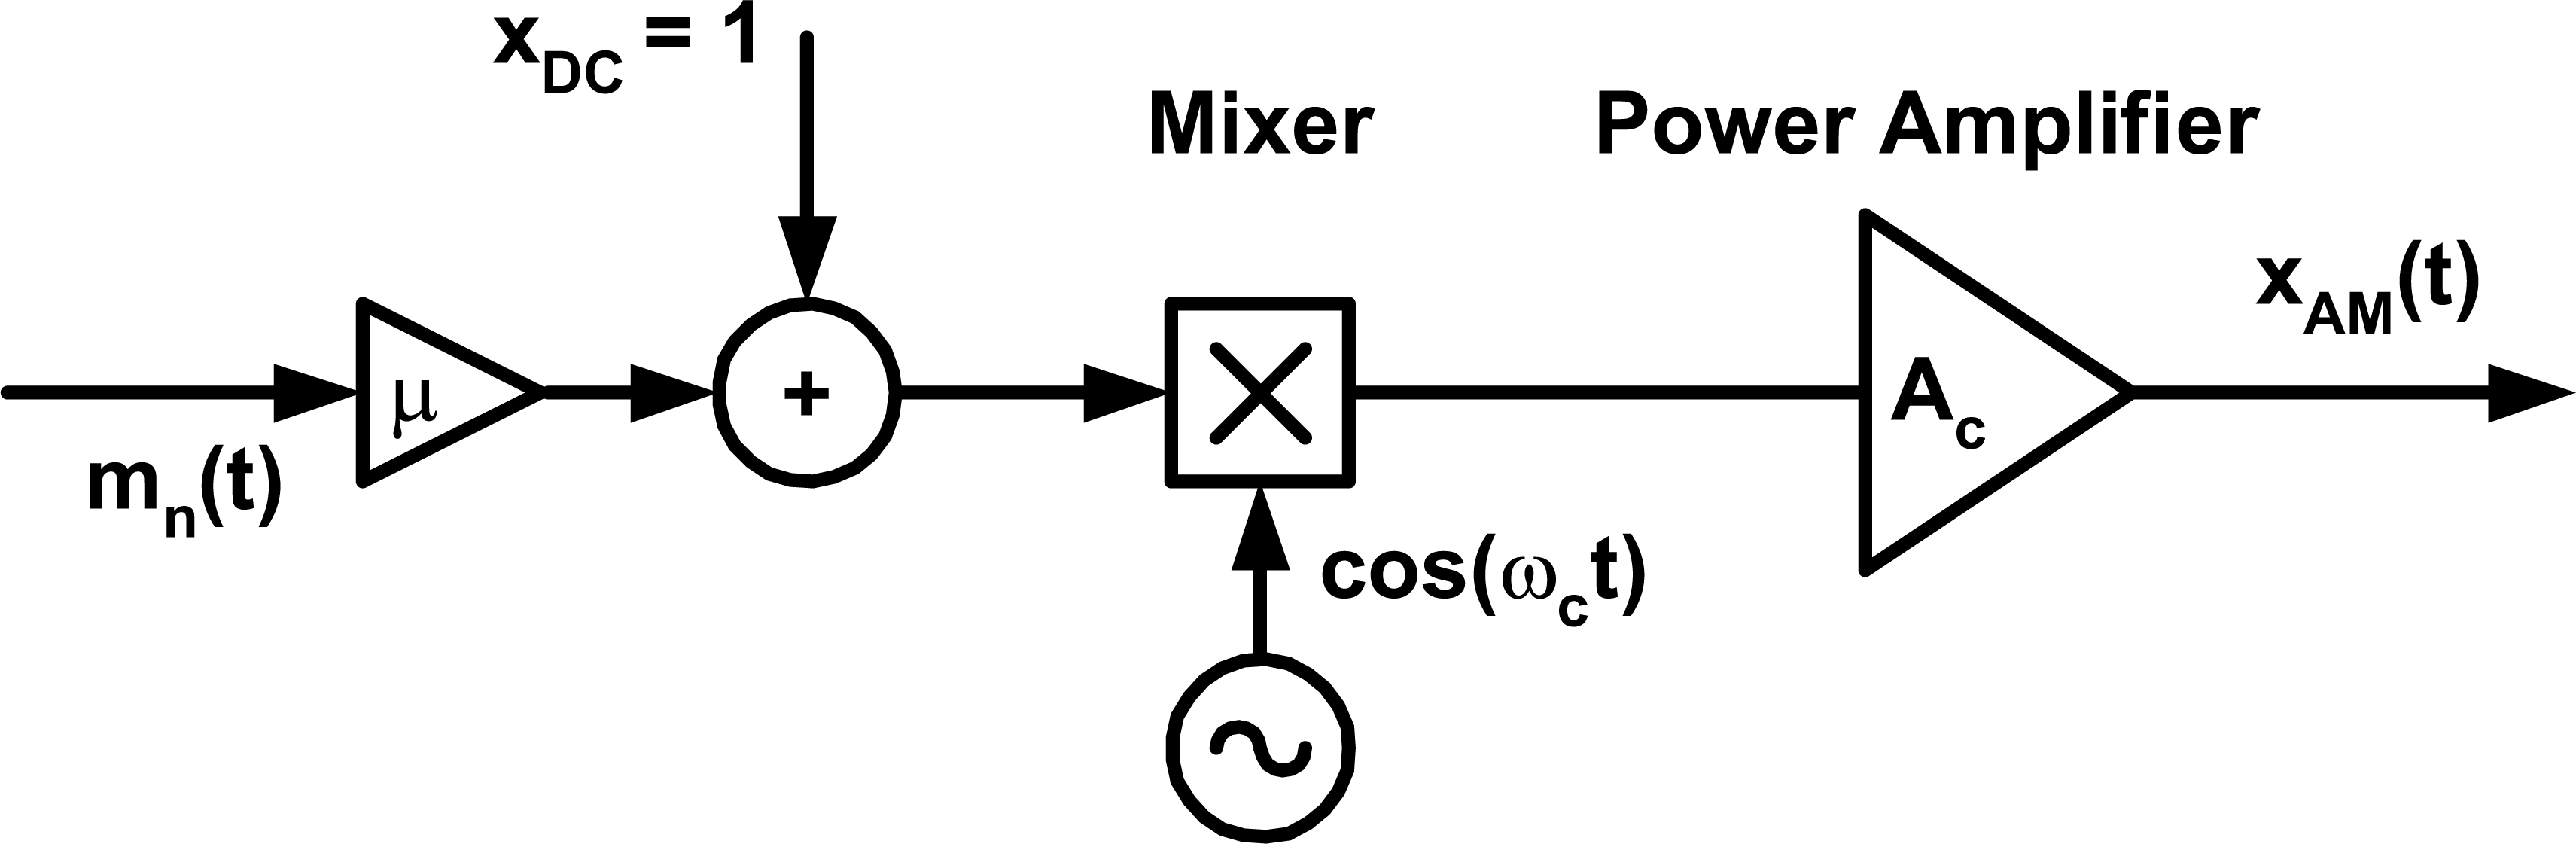
\includegraphics[width=9cm]{bilder/am_oam_modulation.png}
\end{minipage}
\begin{minipage}[]{9cm}
    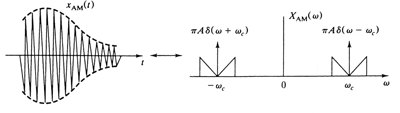
\includegraphics[width=9cm]{bilder/am_oam_spektrum.png}
\end{minipage}\\
Die Bandbreite bleibt gleich wie bei DSB-AM, jedoch befindet sich nun ein grosser Teil der
Signalleistung im Träger. \\
Diese Art von AM hat sich v.a. in füheren Zeiten durchgesetzt, weil die Demodulation mit sehr
wenig Aufwand realisiert werden kann. 

\subsubsection{Demodulation}
\paragraph{Mit Enveloppen Detektor}
Der Enveloppen Detektor braucht nur drei Bauteile, der Schaltungsaufwand ist also
sehr gering.\\
\begin{center}	
      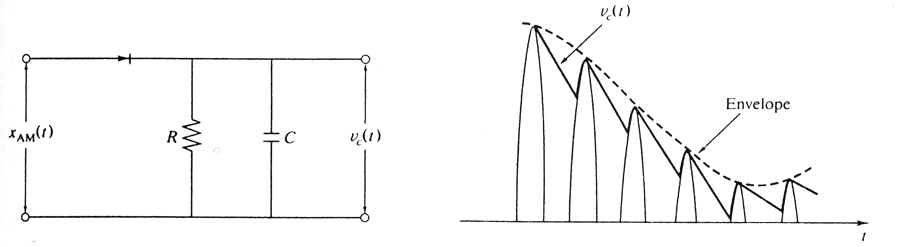
\includegraphics[width=14cm]{bilder/am_oam_enveloppeDetektor.png}
\end{center}
Damit der Envelope Detektor korrekt funktioniert müssen R und C korrekt gewählt werden, es gilt:
$RC \leq \frac{\sqrt{1 - \mu^2}}{\omega_m \mu}$ \\
In der Praxis genügt jedoch das Erfüllen der Bedingung $\frac{1}{\omega_c} \ll \frac{1}{W_M}$,
wobei es sich bei $W_M$ um die Bandbreite des Nachrichtensignals handelt. 

\paragraph{Mit kohärentem (synchronen) Demodulator}
Ordinary AM kann auch mit dem kohärenten Demodulator demoduliert werden
\verweis{am_dsb_modulation}{}:
$y(t) = \frac12 (A + m(t)) = \frac12 m(t) + \frac12 A$ mit nachfolgendem
seriellem Kondensator (Hochpass).


\skriptsubsubsection{Modulationsindex}{46}
Der Modulationsindex $\mu$ ist für AM wie folgt definiert.
$$\mu = \frac{|min\{m(t)\}|}{A_c} = \frac{A_m}{A_c} $$
Um eine Demodulation mit dem Envelope-Detektor zu ermöglichen, muss die Bedingung 
\textbf{$\mu \ll 1$} erfüllt sein. \\
Ist dies nicht der Fall (\textbf{$\mu > 1$}) so spricht man von einer \textbf{Übermodulation} oder
einem  \textbf{übermodulierten Träger}, was in einer Envelope-Verzerrung resultiert. \\
Anbei zwei Fälle zur Veranschaulichung dieser Problematik: Links ($\mu \ll 1$), Rechts ($\mu > 1
\rightarrow $ Übermodulation).

\begin{minipage}[t][2.3cm][c]{9.5cm}
	\begin{center}
      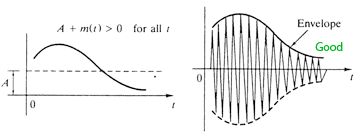
\includegraphics[width=8cm]{bilder/am_oam_enveloppeGood.png}
	\end{center}
\end{minipage}
\begin{minipage}[t][2.3cm][c]{9.5cm}
    \begin{center}
    	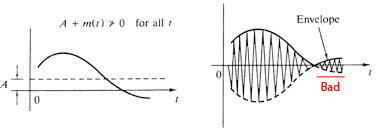
\includegraphics[width=8cm]{bilder/am_oam_enveloppeBad.png}
	\end{center}
\end{minipage}

\skriptsubsubsection{Effizienz / Wirkungsgrad}{55-3.4}
Unter der Effizienz $ \eta $ der gewöhnlichen AM versteht man das Verhältnis von der Signalleistung
$P_s$ der beiden Seitenbänder zur Gesamtleistung $P_t$ des AM-Signals.

$$ P_c = \frac{A_c^2}{2} \quad \text{und} \quad P_t = \frac{A_c^2}{2} + \frac{\mu^2 A_c^2}{4}
\quad \Longrightarrow \quad \eta = \frac{P_s}{P_t} = \frac{P_t - P_c}{P_t} =
\frac{\mu^2\cdot P_m}{1+\mu^2 \cdot P_m} =
\frac{k^2\cdot P_m}{1+k^2 \cdot P_m}$$

Die maximale Effizienz (bei $\mu = 100\% $) beträgt nur gerade $ \eta = 33\% $. Bei $\mu = 50\% $
sind es noch bescheidene $\eta = 11.1\% $.

\skriptsubsection{SSB: Einseitenband (Single-Sideband)-AM}{47}
Sowohl Gewöhnliche AM als auch DSB verschwenden Bandbreite, weil diese immer beide Seitenbänder
übermitteln. \\
Ist dies nicht der Fall - wird also \textbf{nur ein Seitenband} übertragen - so spricht man von
Einseitenband-AM. Deren Vorteil liegt in der Reduktion der Bandbreite, was aber auch den Nachteil
- Die Komplexität der Implementation - mit sich bringt.

\subsubsection{Modulation}
\textbf{Phasenverschiebung \formelbuch{59-3.8}}  \\
\begin{minipage}[t][3.7cm][c]{7.5cm}
    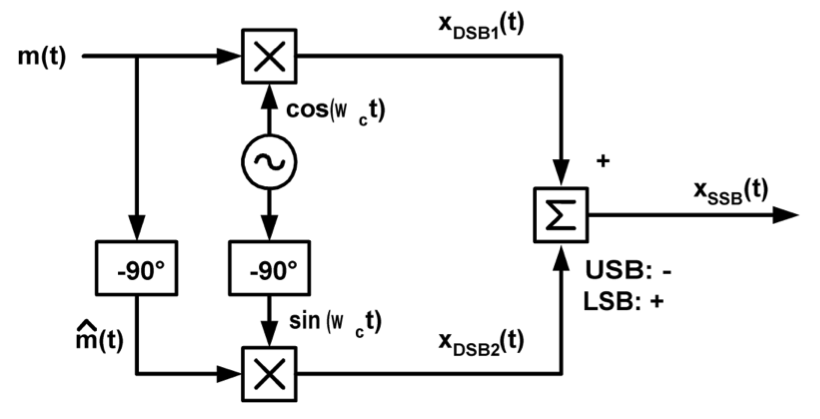
\includegraphics[width=7cm]{bilder/am_ssb_modulationPhasenshifter.png}
\end{minipage}
\begin{minipage}[t][3.7cm][c]{10.5cm}	
	Des weiteren bieter sich die Möglichkeit ein SSB-Signal mit Hilfe von 
	$ - 90^{\circ} $-Phasenschiebern zu generieren, {\small siehe
	\ref{lti_quadratur} Quadraturfilter (S. \pageref{lti_quadratur}) \&
	\ref{lti_hilbert} Hilbertransformation (S. \pageref{lti_hilbert})}.\\
	Die Amplitude des SSB-Signals ist im Spektrum \textbf{gleich hoch} wie die des
	Nachrichtensignals.\\ 
	$+$: Lower Sideband; \qquad $-$: Upper Sideband
\end{minipage}

\textbf{Frequenzdiskriminierung} \\
\begin{minipage}[t][2cm][c]{5.5cm}
    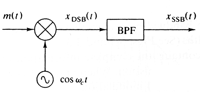
\includegraphics[width=5cm]{bilder/am_ssb_modulationFilter.png}
\end{minipage}
\begin{minipage}[t][2cm][c]{12.5cm}	
	Hierbei wird ein DSB-Signal mit einem Hoch- oder Tiefpass gefiltert, sodass ein SSB-Signal
	resultiert. Diese Methode ist in der \textbf{Praxis unüblich}, da sehr steile Filter benötigt
	werden.\\
	Die Amplitude des SSB-Signals ist im Spektrum \textbf{halb so hoch} wie die des
	Nachrichtensignals.
\end{minipage}

\subsubsection{Demodulation}
Diese erfolgt wie bei DSB-AM \verweis{am_dsb_modulation}{Modulation DSB-AM}.\\


\skriptsubsection{VSB: Restseitenband (Vestigial-Sideband)-AM)}{49}
\subsubsection{Modulation}
\begin{minipage}[t][2.2cm][c]{5.5cm}
    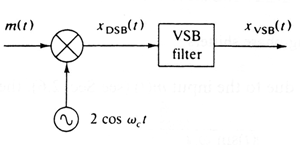
\includegraphics[width=5cm]{bilder/am_vsb_modulator.png}
    %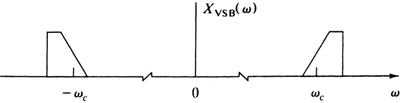
\includegraphics[width=7cm]{bilder/am_vsb_spektrum.png}
\end{minipage}
\begin{minipage}[t][2.2cm][c]{12.5cm}	
Restseitenband-AM ist sozusagen die praktische Realisierung der Frequenzdiskriminierungsmethode bei
SSB. Es wird ein DSB-Signal mit einem Restseitenbandfilter (sideband-shaping filter) gefiltert,
wodurch schlussendlich das VSB-Singal resultiert mit etwa 1.25-facher Bandbreite von SSB.
$ \qquad  W_{VSB} \approx 1.25 \cdot W_{SSB} $
\end{minipage}
\begin{center}
    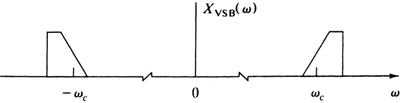
\includegraphics[width=8cm]{bilder/am_vsb_spektrum.png}
\end{center}

\subsubsection{Demodulation}
Auch diese Art von AM kann mit einem kohärenten Demodulator demoduliert
werden \verweis{am_dsb_modulation}{Modulation DSB-AM}.\\
Für eine verzerrungsfreie Demodulation ist erforderlich, dass $H(\omega +
\omega_c) + H(\omega - \omega_c) = const$ für $|\omega| \leq |\omega_m|_{max}$.



\skriptsubsection{QAM: Quadratur(Quadrature)-AM}{64-3.15}
Hierbei werden zwei orthogonale Träger ($\sin, \cos$) verwendet, sodass zwei Nachrichtensignale
zusammen übertragen werden können. Dies ist zwar technisch aufwendiger, jedoch wird die Bandbreite
doppelt genutzt. \\
Bei der Demodulation muss darauf geachtet werden, dass der Demodulator synchronisiert ist. Ist dies
nicht der Fall, so kann sich bei grösserer Phasenabweichung das andere Nachrichtensignal
``einschleichen''.
\begin{center}
    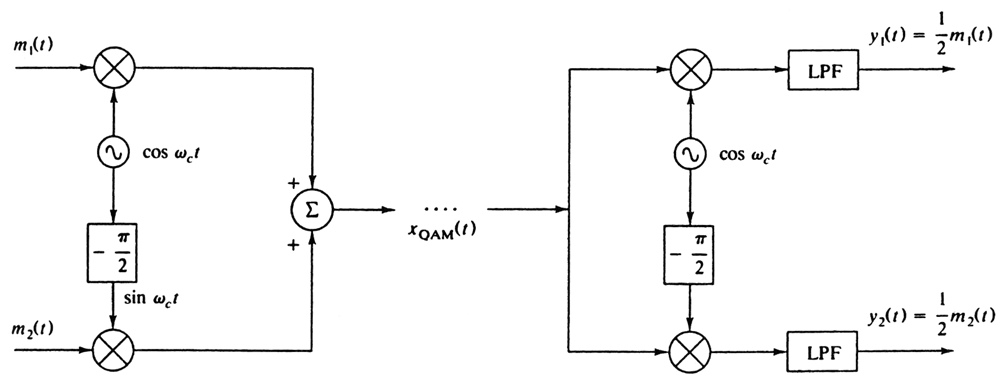
\includegraphics[width=14cm]{bilder/am_qam_modulatorDemodulator.png}
\end{center}
